A
% intro %

In high	energy physics, we need two things: acceletors to create particles and detectors to detect them. LHC is one of the biggest acceleratos we have today, and one on if its general detectors is (CMS) which is related to this thesis.This chapter provides details about LHC, protons journey at LHC, and discribtion of CMS detector.   

%................................
%\section{The large hadron collide}

The large hadron collider is the most powerful particle accelerator in the world. From its name “Large” refer to its big size which is about 27km in circumference and “Hadron" because it accelerates particles like protons or ions which are known as hadrons.Lastly, "Collider" because the particles traveling into two beams in opposite directions, are made to collide at four points around LHC ring.

The LHC is a part of the CERN accelerator complex and sits in a tunnel 100 meters underground at CERN, the European Organization for Nuclear Research, on the border of Switzerland and France near Geneva, Switzerland.

The CERN accelerator complex is a succession of machines where each machine accelerates a beam of particles to a given energy before injecting the beam into the next machine in the chain. LHC is the last element of this chain where it is designed to collide particles at COM energy up to 14 TeV.

The LHC is made of eight arcs and eight ‘insertions. The arcs contain the dipole ‘bending’ magnets. The layout of the straight section depends on the specific use of the insertion: physics (beam collisions within an experiment), injection, beam dumping or beam cleaning.

At the LHC we have 9 experiments:
ALICE (study heavy ion collisions, QGP) ATLAS, CMS  (general purpose detectors) LHCb (study matter – antimatter asymmetry) ,LHCf (shares intersection with ATLAS),TOTEM (shares intersection with CMS) MoEDAL-MAPP, (shares intersection with LHCb), FASER,SND@LHC.

\subsection{The journey of protons in the LHC}

It all starts from a compressed tank of hydrogen that is connected to source chamber of the linear accelerator.
The Linear accelerator 4 (Linac4) is designed to boost negative hydrogen ions (H with extra electron) to high energies (initial to 1/3 C).Then the particles are fed to the booster stage. (Proton Synchrotron Booster – PSB).at the PSB injection point a stripping foil will strip the electrons off the hydrogen anions creating protons that are accumulated as beam bunches in the four PSB rings.

These proton bunches are then recombined at the exit of the PSB and further transferred down theCERN injector chain (accelerated to 91.6 of C).After that the beam is sent to Proton synchrotron (PS) where the increase of energy does not transfer to velocity.
Instead, it will increase the relativistic mass (accelerated to 99.9 of C).

Then the protons go to the super proton synchrotron. (SPS). Finally, at the LHC has two vacuum pipes where the protons will be going into different directions. 27 km ring of superconducting magnets (keep protons in the ring) that also has  accelerating structures (radio frequency cavities) to boost the energy. The LHC’s RF cavities bring the 450 GeV energy  of the particles (1 GeV = 1 billion electron volts) to 6.5 TeV source.

The maximum energy is reached in around 20 minutes with the bunches having passed through the RF cavities more than 10 million times.There are 4 points where the protons are collided. CMS is one of the them, where this thesis is focus on.

\section{CMS Detector}

CMS detector is one of the main detectors at the LHC. It is a general-purpose detector. its physics program rang from studying the Standard Model (including the Higgs boson) to searching for extra dimensions and particles that could make up dark matter.
CMS stands for Compact Muon Solenoid. measure the position and energy of all particles that comes from the collision. This detector weights 14,000-tonne but it is quite compact for all the detector material it contains. It is at 15 m high  and 21 m long.
CMS is it isdesigned to detect muons very accurately. Also, it has the most powerful solenoid magnet ever made.

The design of CMS and its subdetectors are based on the geometry of its solenoid magnet. some of the subdetectors are located inside the magnet while the rest are outside the magnetic field. Inside starting from the closest to the beam pipe we have: Silicon tracker (Silicon pixel, Silicon strips) designed to minimally interact with particles. ECAL & HCAL will stop and absorb the particles completely (calorimeters).  Outside the magnet there are some of HCAL subdetectors a\
nd muon systems.


\subsection{Superconducting Magnet}
It is superconducting magnet that produces 3.8 T magnetic field inside a solenoid and quickly drops off outside it. Thi\
s magnetic field is used to determine the momenta of charged particles since the trajectories of the particles bend in \
the field.

\subsection{Inner Tracker}
the first subdetector particles created from the collision will interact with after leaving the beam pipe is the tracker. The most inner parts of the CMS detector are: the pixels, silicon microstrip detectors that surrounds the pixels.

Main function of the tracker is to measure the curvature of charged particles with pt > 1 GeV. From which we can use to determine the momentum. When a charged particle goes through the tracker it will leave a hit (tiny signal that will later be amplified and detected) in the tracker layers. These hits could be aligned to get the trajectory of the particle. The signals will be stored for microseconds and then processed before being sent to a laser to be converted to an infrared pulse Which will be transmitted for analysis.

The pixel detector:
It is also the closest detector to the beam pipe. It has 4 cylindrical layers at (3,7,11,16 cm) . Each of the four layers is composed of individual silicon module (? How many), splitted into little silicon sensors (pixels).  Each of these silicon pixels is 100µm by 150µm.

The silicon strips
After the pixels the particles go through the silicon strip detector, which has10 layers. (130 cm~ 1.3m). 4 inner barrel layers (TIB) with two inner endcaps (TID) each has 3 small disks. Then we have 6 outer barrel layer (TOB) surrounds both TIB, TID with two endcaps (TED) closing off the tracker. this part contains 15,200 highly sensitive modules with a total of about 10 million detector strips.

(insert real/sketch updated picture of each subdetector)


\subsection{Electromagnetic Calorimeter}
it is a homogeneous calorimeter made of lead tungstate crystals. Measures the energy of electrons and photons. It is made up of a “barrel” section and two “endcaps”, that would form a layer between the tracker and the HCAL.
tungstate crystals are heavier than stainless steel but it is transparent. It scintillates when electrons and photons pass through it. Which will produce light that is that is proportion to the particle energy.

glued onto the back of each of the crystals a Photodetectors, which have been especially designed to work within the high magnetic field, will detect the scintillation light and convert it to an electrical signal that is amplified and sent for analysis.

The barrel region: consists of 61,200 crystals formed into 36 “supermodules”, each weighing around three tonnes and con\
taining 1700 crystals. Here each crystal (2.2 x 2.2 x 23 cm). it can contain more than 98 of the electrons and photons \
energy.

The endcap regions close off the barrel at each end and are made  up of almost 15,000 more crystals. each crystal (3 x 3\
 x 22 cm) which corresponding to 24.7 radiation lengths. For more precision, the ECAL also contains a pre shower detector that is Finer grained detector and located before either endcap disk.  has two layers, each layer is made of two orthogonal layers of silicon sensors, interspersed with lead layers that serve to generate electromagnetic showers. This detector serves two goals Find the photons decaying form a neutral pion to discriminate them from prompt photons.  Indicate the presence of an electron or a photon in the ECAL be requiring a related signal in the pre shower.


 (what pics to include?)

 \subsection{Hadronic Calorimeter}

 Hermetic & sampling calorimeter
It is “hermetic” makes sure it captures, to the extent, every particle emerging from the collisions. It HCAL measures directly the energy of “hadrons”. Like: neutrons, Pions and kaons and indirect the presence of non-interacting, uncharged particles such as neutrinos by seeing the imbalance in the momentum and energy (measured in the sideways “transverse” direction relative to the beam line).

HCAL is also a sampling calorimeter made of alternating layers of “absorber” (dense material - brass or steel) and fluo rescent “scintillator” (tiles of plastic) that produce a rapid light pulse when the particle passes through.
the HCAL is organized into: Barrel region: (HB) these form the last layer of detector inside the magnet coil while a few additional layers the outer barrel (HO), sit outside the coil, ensuring no energy leaks out the back of the HB undetected. endcap regions measure particle energies as they emerge through the ends of the solenoid magnet. Forward sections  positioned at either end of CMS; to pick up the myriad particles coming out of the collision region at shallow angles relative to the beam line, these receive the bulk of the particle energy contained in the collision so they must be very resistant to radiation and use different materials to the other parts of the HCAL.

When a hadronic particle hits a plate of absorber, in this case brass or steel, an interaction can occur producing numerous secondary particles. As these secondary particles flow through successive layers of absorber. they too can interact and a cascade or “shower” of particles results.

As this shower develops, the particles pass through the alternating layers of active scintillation material causing the\
m to emit blue-violet light. Within each tile tiny optical absorb this light. clear optic cables then carry the light a\
way to readout boxes located at locations within the HCAL volume. signals from successive tiles, one behind the other, \
are added optically to form “towers”. These summed optical signals are converted into fast electronic signals by photos\
ensors.

(insert sketch that shows the subdetectors of the HCAL)

\subsection{Muon Detector}
Detecting muons is one of CMS’s most important tasks. unlike most particles muons are not stopped by any of CMS’s calorimeters.That is why chambers to detect muons are placed atthe very edge of the experiment where they are the only particles likely to register a signal.muon chambers that include: Drift tubes (DTs) and cathode strip chambers (RPCs) are arranged in concentric cylinders around the beam line in the barrel region. In endcap region we have CSCs and resistive plate chambers (RPCs) which make u\
p the “endcaps” disks that cover the barrel (add gas electron multiplier chambers (GEMs))
the muon is measured by fitting a curve to hits among the four muon stations (MS) which sit outside the magnet coil and\
 are interleaved with iron “return yoke” plates.
 (Insert picture that shows the placement of each type in both regions)

 


 %------------ figures ------------%
\begin{figure}[t!]
\centering
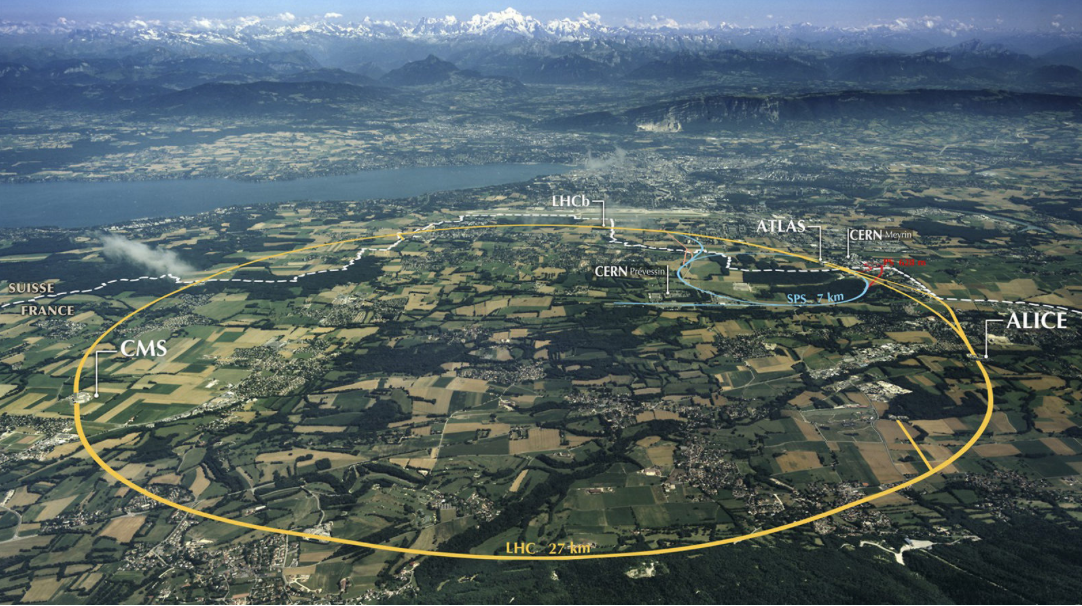
\includegraphics[width=0.99\textwidth]{figures/LHC_location.png}}
\caption[location of the LHC]{}. %Figure source~\cite{SMtable}.
%\label{fig:SMParticles}}
\end{figure}

\begin{figure}[t!]
\centering
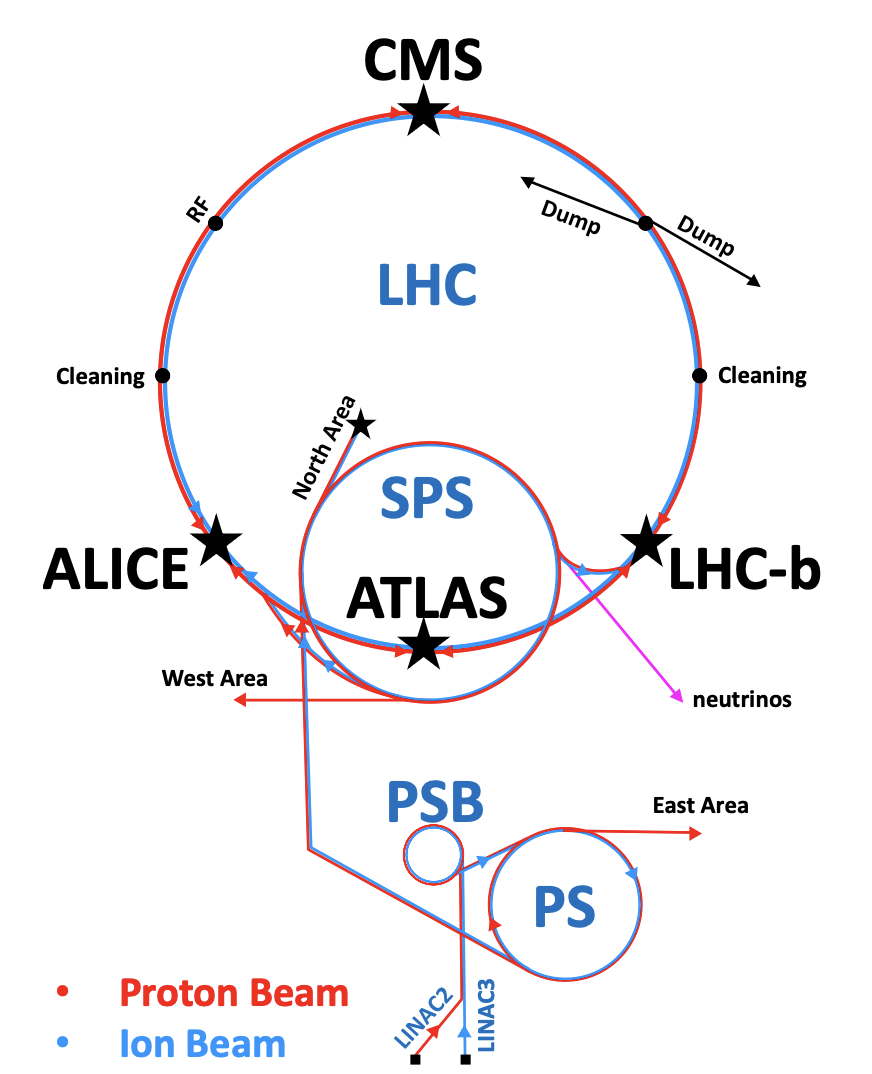
\includegraphics[width=0.99\textwidth]{figures/acceleration_chain.png}}
\caption[acceleration complex]{}. %Figure source~\cite{SMtable}.
%\label{fig:SMParticles}}
\end{figure} 
   

